\chapter{Gerarchie di Memoria e Architettura con Cache}

\section{Gerarchie di Memoria}

La grande quantità di dati, normalmente presente in un sistema di elaborazioni, viene memorizzata su sopporti con caratteristiche molto diverse tra loro in termini di tempo di accesso, capacità e costo.\
Diremo che esiste una \textit{gerarchia di memoria}, nella quale al \textit{livello più alto} stanno i dispositivi di memoria più capaci, più lenti e meno costosi.\
Man mano che si scende di livello nella gerarchia, i supporti hanno capacità più piccola, tempo di accesso sempre più basso e costo per bit sempre più grande.

\textit{Salendo di livello nella gerarchia di memoria}, il tempo di accesso aumenta non solo per le \textit{caratteristiche intrinseche dei supporti di memorizzazione}, ma anche per i ritardi crescenti nelle \textit{comunicazioni} necessarie per richiedere le informazioni e per farle pervenire ove devono essere elaborate.

Di tutta l'enorme massa d'informazioni disponibili in un sistema, istante per istante solo una piccolissima parte viene utilizzata dall'elaborazione in corso; d'altronde, questa parte varia \textit{dinamicamente} durante l'elaborazione stessa.\
L'obiettivo di una gerarchia di memoria, che possa dirsi ``efficiente'', è quello di riuscire, istante per istante, a mantenere nei livelli più bassi tutte e sole le informazioni strettamente indispensabili all'elaborazione corrente.\
Ciò comporta un \textit{continuo spostamento} d'informazioni attraverso i livelli della gerarchia di memoria:\ quelle che, man mano, si rendono sempre più utili scendono di livello, andando a sostituirne altre, ritenute momentaneamente meno utili, le quali vengono riportate nei livelli più alti.

\subsection{Gerarchie di memoria con paginazione}

Consideriamo due livelli contigui, $\mathrm{M}_1$ e $\mathrm{M}_2$, nella gerarchia di memoria, con $\mathrm{M}_2$ livello più alto.\
Il sistema genera indirizzi appartenenti a $\mathrm{M}_2$; questi vengono tradotti in indirizzi di $\mathrm{M}_1$ se l'informazione riferita in $\mathrm{M}_2$ è attualmente allocata in $\mathrm{M}_1$, altrimenti viene generata un'eccezione che provoca la riallocazione di $\mathrm{M}_1$.

Il metodo che sta alla base della maggior parte delle applicazioni del concetto di gerarchia di memoria è
quello della \textbf{paginazione}.\
Lo spazio di $\mathrm{M}_1$ e quello di $\mathrm{M}_2$ \textit{vengono pensati} come suddivisi in blocchi, o pagine, di ampiezza fissa composti di informazioni a indirizzi contigui.

Indicheremo con
\begin{itemize}
    \item $\gamma$ la capacità complessiva di uno spazio di memoria;
    \item $\sigma$ l'ampiezza di una pagina nella gerarchia di memoria considerata;
    \item $v = \gamma/\sigma$ il numero di pagine componenti quello spazio di memoria nella gerarchia considerata.
\end{itemize}

\subsection{Paginazione su domanda}

Nel metodo detto della \textit{paginazione su domanda}, quando, nel tentativo di tradurre un indirizzo $n$ di $\mathrm{M}_2$ viene generato un fault, allora l'\textit{intera pagina} che contiene inf[n] viene trasferita da $\mathrm{M}_2$ a $\mathrm{M}_1$ provocando il \textit{rimpiazzamento} di una pagina già presente in $\mathrm{M}_1$.\
L'efficacia di questo metodo si basa su due proprietà dei programmi che si verificano di frequente:

\begin{itemize}
    \item la \textit{località}, o località temporale, secondo la quale i riferimenti generati da un processo tendono ad accentrarsi, in ogni istante, in gruppi relativamente piccoli di indirizzi tra loro vicini, e tali gruppi tendono a cambiare in modo relativamente lento e intermittente;
    \item il \textit{riuso}, o località spaziale, secondo la quale, nel corso dell'esecuzione di un processo, queste tende a riferirsi più volte a certe locazioni (cicli iterativi, procedure, riassegnamenti di una variabile).
\end{itemize}

\noindent In tal modo, una volta che una pagina è stata trasferita in $\mathrm{M}_1$, questa tende a essere riferita più volte.\
Se in $\mathrm{M}_1$, è presente un numero sufficientemente alto di pagine di $\mathrm{M}_2$, la probabilità che si generi un fault (\textbf{probabilità di fault}) può essere mantenuta a un valore basso a piacere.

La probabilità di fault, $h$, è in genere una funzione della capacità del livello più basso della gerarchia, dell'ampiezza del blocco, e della politica di rimpiazzamento delle pagine.

Le seguenti figure mostrano qualitativamente l'andamento di $h$ al variare di $\gamma$, per $\sigma$ costante, e di $h$ al variare di  $\sigma$, $\gamma$ con costante:

\begin{figure}[H]
    \centering
    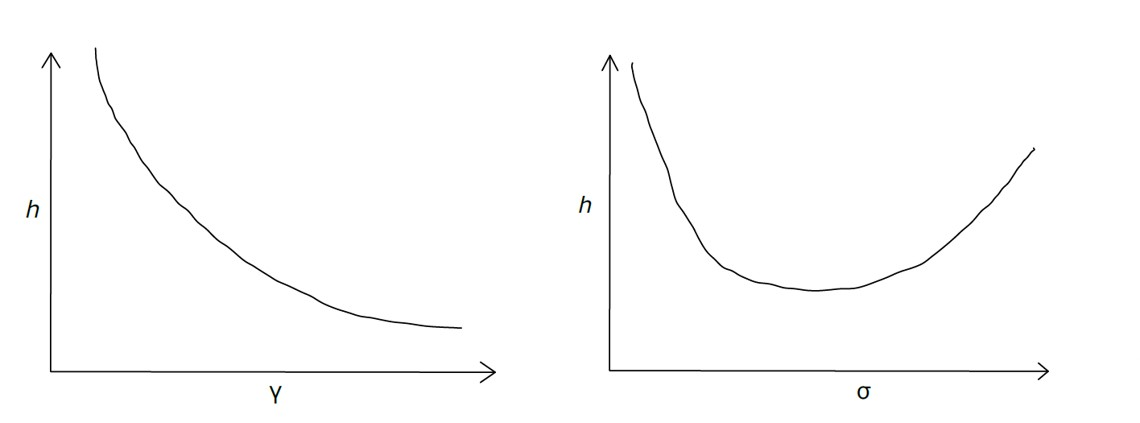
\includegraphics[width=\textwidth]{immagini/Fault.jpg}
\end{figure}

\subsection{Insieme di lavoro}

In una gerarchia di memoria $\mathrm{M}_2\textrm{-}\mathrm{M}_1$, l'insieme di lavoro di un programma (processo) è definito come l'\textit{insieme di pagine} (\textit{blocchi}) che, \textit{se presenti contemporaneamente in $\mathrm{M}_1$, rendono minima la probabilità di fault}.\
L'insieme di lavoro va considerato sia in termini di quante pagine che di quali pagine devono essere possibilmente presenti in $\mathrm{M}_1$ contemporaneamente.

L'obiettivo di una gestione efficiente di una gerarchia di memoria è quello di individuare l'insieme di lavoro e cercare di mantenerlo in $\mathrm{M}_1$.\
A questo scopo, occorre cercare di sfruttare al meglio le proprietà di \textit{località} e, in particolare, di \textit{riuso} di ogni programma.

\section{Gerarchia Memoria Virtuale - Memoria Principale}

\subsection{Spazi di indirizzamento}

Durante la fase di traduzione, il compilatore provvede a scegliere gli indirizzi di memoria per le istruzioni e per i dati di $Q$.\
Viene così definito lo \textit{spazio di indirizzamento logico del processo}, $N$, cioè l'insieme di tutti gli indirizzi, noti a tempo di compilazione e generati dal processore a tempo di esecuzione.

Chiamiamo \textit{spazio di indirizzamento fisico}, $M$, l'insieme degli indirizzi di memoria principale (\textit{indirizzi fisici}) assegnati a un processo quando viene allocato in memoria principale.\
$M$ può coincidere o essere un sottoinsieme dei possibili indirizzi della memoria principale.

\subsection{Allocazione della memoria principale}

Nel caso di allocazione statica della memoria principale, $N$ e $M$ coincidono.\
Per essere eseguito, tutto il processo è interamente caricato da memoria secondaria a memoria principale in un'area nota.

Nel caso di allocazione dinamica della memoria principale, lo spazio $M$ assegnato al processo varia a tempo di esecuzione sia in posizione sia in quantità.\
In generale, non tutto $N$ è allocato contemporaneamente in memoria principale, ma solo una sua parte, possibilmente quella che, istante per istante, permette al processo di reperire la maggior parte delle informazioni (istruzioni e dati) in memoria principale.\
La parte di $N$ allocata in memoria principale varia a tempo di esecuzioni, così come la zona di memoria principale in cui allocare \textit{N}.\
Inoltre, in generale tale zona non è contigua, anche nel caso che $N$ lo sia.

Per un processo $Q$ deve essere definita una funzione di rilocazione, o funzione di traduzione degli indirizzi:
\[\mu_Q: N \rightarrow M\]
La funzione di traduzione degli indirizzi $\mu_Q$, implementata con la Tabella di Rilocazione, viene aggiornata e valutata a tempo di esecuzione per ogni indirizzo logico generato dal processo $Q$ in esecuzione sul processore.\
Ciò avviene con l'ausilio di supporti hardware-firmware particolarmente efficienti:\ l'unità \textit{MMU} che, facente parte della CPU, fa da tramite tra processore e memoria principale, provvedendo a tradurre gli indirizzi da logici a fisici in un solo ciclo di clock; nel caso che $\mu_Q$ non sia definita, \textit{MMU} restituisce l'eccezione al processore.

\subsection{Creazione di processi, caricamento, e commutazione di contesto}

Quando un processo $Q$ esegue una primitiva di \textit{creazione} di un altro processo $R$, questa provoca un \textit{caricamento} di $R$, cioè il trasferimento di informazioni di $R$ da memoria secondaria a memoria principale.\
Una volta creato, $R$ viene posto nello \textit{stato di pronto}.

Il file, che rappresenta il prodotto della traduzione dal programma al processo $R$, contiene diverse informazioni, sotto forma di opportune strutture dati, che verranno utilizzate da funzionalità del supporto durante l'evoluzione del processo stesso:\ in particolare, la struttura dati \textit{descrittori di processo} (\textit{PCB}).

\textit{Il PCB viene inizializzato a tempo di compilazione}, in particolare assegnando i valori costanti con cui inizializzare i registri generali e il contatore istruzioni.

Quando il processo $R$ viene creato, in memoria principale viene compilato anche il suo PCB con il valore che è stato inizializzato a tempo di compilazione.

Quando verrà il turno di $R$ a passare in esecuzione sul processore, ha luogo \textit{la commutazione di contesto}:

\begin{itemize}
    \item l'immagine di RG e di IC viene copiata dall'area facente parte del PCB\textsubscript{R} nei registri RG e nel registro IC.\ In tal modo:
          \begin{itemize}
              \item i registri sono inizializzati come stabilito a tempo di compilazione,
              \item la prima istruzione da eseguire sarà quella all'indirizzo logico di R, stabilito a tempo di compilazione, che è stato scritto in IC;
          \end{itemize}
    \item il processo ($T$) che esce dallo stato di esecuzione provvede a salvare nel proprio $\mathrm{PCB}_T$ i valori correnti di RG e IC.\ In tal modo, quando successivamente \textit{T} tornerà in esecuzione, RG e IC verranno ripristinati con le rispettive immagini presenti nel $\mathrm{PCB}_T$, esattamente secondo lo schema descritto precedentemente, in modo che $T$ possa riprendere l'esecuzione a partire dall'ultima eseguita prima di sospendersi e con i contenuti dei registri generali presenti prima di sospendersi.
\end{itemize}

\subsection{Allocazione dinamica della memoria con paginazione}

Il processo, una volta creato, in ogni istante risulta allocato in uno spazio fisico di memoria principale, che in generale non è né contiguo né completo:\ non tutto il processo risiede contemporaneamente in memoria, e la parte che vi risiede è distribuita in \textit{blocchi}, o \textit{pagine}, di ampiezza fissa e al loro interno contigue, ma sparse in zone diverse della memoria.

In un caso tipico, una pagina è ampia 1K parole con indirizzi logici di 32 bit.\
L'indirizzo logico può dunque essere visto come composto dalla concatenazione di due campi:\ quello dei bit più significativi fornisce l'\textit{identificatore di pagina logica}, IPL, e quello dei bit meno significativi l'\textit{indirizzo all'interno della pagina} o \textit{displacement}.

La funzione di rilocazione del processo $Q$, $\mu_Q$, viene implementata mediante una tabella, detta Tabella di Rilocazione del processo, $\mathrm{TABRIL}_Q$, il cui contenuto è inizializzato a tempo di caricamento/creazione e varia durante l'esecuzione del processo in seguito all'allocazione dinamica di pagine.

\textit{Attraverso la Tabella di Rilocazione la funzione di rilocazione viene applicata alle pagine}.\
L'entrata $i$-esima della Tabella di Rilocazione contiene, tra le altre informazioni:

\begin{itemize}
    \item un \textit{bit di presenza}, \texttt{PRES}, che, se a uno, indica che la pagina logica $i$-esima è presente in memoria principale;
    \item un \textit{identificatore di pagina fisica}, \texttt{IPF}, cioè l'identificatore della pagina di memoria principale dove risiede la pagina logica $i$-esima nel caso che $\mathtt{PRES} = 1$.
\end{itemize}

\begin{figure}[H]
    \centering
    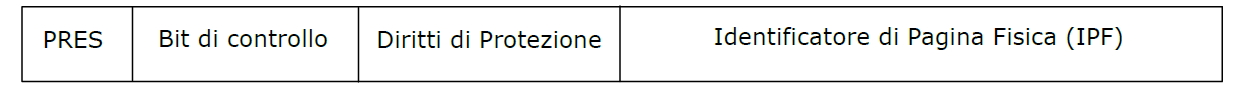
\includegraphics[width=\textwidth]{immagini/Tabril.png}
\end{figure}

\noindent Indichiamo con $x^{\circ} y$ il concatenamento dei valori $x$, $y$ in una stessa unità di informazione.\
Dato l'indirizzo logico $\mathrm{IPL}^{\circ}\mathit{displ}$ generato dal processo $Q$, se $\mathrm{TABRIL}_Q[\mathrm{IPL}].\mathtt{PRES} =1$, allora l'indirizzo fisico corrispondente è dato da $\mathrm{TABRIL}_Q[\mathrm{IPL}].\mathtt{IPF}^{\circ}\mathit{displ}$.

Se $\mathrm{TABRIL}_Q[\mathrm{IPL}].\mathtt{PRES} = 0$, allora viene generata l'eccezione di fault di pagina.

Nello schema di TABRIL è anche indicato il campo ``Bit di controllo'' contenente un bit per ricordare se la pagina è stata modificata e informazioni per implementare la politica di rimpiazzamento.\
Quest'ultima politica, \textit{eseguita dalle funzionalità di gestione della memoria in seguito all'eccezione di fault di pagina}, ha come scopo la scelta della pagina da sostituire; \textit{la scelta che mediamente fornisce il risultato migliore, agli effetti della riduzione della frequenza dei fault di pagina} è la \textbf{LRU} (Least Recently Used).

\subsection{MMU}

La traduzione dell'indirizzo logico e l'eventuale generazione di eccezioni di fault di pagina sono implementate a hardware-firmware nell'unità \textit{MMU} facente parte della CPU.

Al processore P non è visibile come avviene la traduzione degli indirizzi, ma deve comunque essere noto l'\textit{esito} di ogni accesso in memoria.

Per effettuare efficientemente la traduzione dell'indirizzo, \textit{MMU} deve disporre di risorse hardware opportune.\
Occorre allora realizzare in hardware una \textit{tabella accedibile per contenuto}:\ questo componente è chiamato \textbf{Memoria Associativa} (MA) ed è costituita da $C$ registri, ognuno contenente una \textit{chiave}, e altrettanti contenenti i corrispondenti \textit{valori}.

Le uscite dei registri-chiave sono ingressi di $C$ confrontatori, il cui secondo ingresso è costituito dalla \textit{chiave Key} con la quale si vuole effettuare la ricerca.\
Quindi viene effettuato il confronto \textit{simultaneo} di \textit{Key} con tutte le Chiavi in tabella.\
Uno dei confronti è positivo, allora l'indice del registro-chiave relativo fornisce univocamente l'indirizzo della RAM dalla quale leggere il Valore corrispondente a \textit{Key}; in caso di tutti i confronti negativi, l'evento negativo viene segnalato attraverso il valore di un bit di Fault.

Una parte di Tabella di Rilocazione TABRIL è mantenuta, dinamicamente, nella Memoria Associativa MA nella PO della \textit{MMU}.\
\textit{Le chiavi sono gli identificatori di pagina logica IPL}, mentre \textit{i valori sono i corrispondenti contenuti TABRIL[IPL] della Tabella di Rilocazione}.

Normalmente, si mantengono in MA le entrate di TABRIL \textit{usate più di recente}:\ questo permette di rendere trascurabile la probabilità che l'entrata di interesse non risieda in MA.\
In caso che venga generato un fault di MA, \textit{MMU} provvede a copiare in MA l'entrata di TABRIL corrispondente alla pagina logica riferita, sostituendo l'entrata usata meno di recente, per questa ragione all'atto della commutazione di contesto, quando viene posto in esecuzione il processo $Q$, \textit{l'indirizzo di} $\mathrm{TABRIL}_Q$ deve essere comunicato a \textit{MMU}, che lo mantiene in un suo registro interno.

\section{Architettura con cache}

\subsection{Struttura della CPU con cache}

\begin{figure}[H]
    \centering
    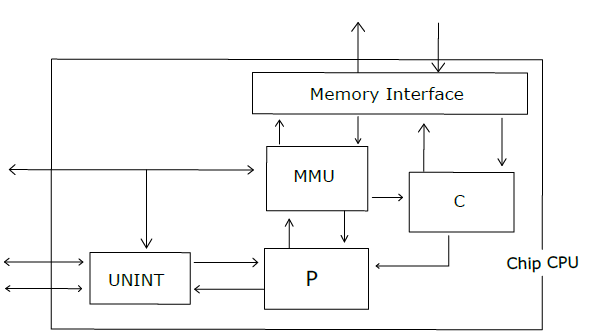
\includegraphics[width=0.7\textwidth]{immagini/CPU_cache.png}
\end{figure}

\noindent Nel caso di successo nella rilocazione dell'indirizzo logico (di memoria virtuale), \textit{MMU} passa la richiesta con l'indirizzo fisico (di memoria principale) all'unità cache $C$.\
Questa provvede \textit{all'ulteriore traduzione da indirizzo di memoria principale a indirizzo di memoria cache}, nel caso che la funzione di traduzione sia definita; in caso di insuccesso (cache \textit{fault}) ha luogo il \textit{trasferimento} del blocco di memoria principale richiesto in uno dei blocchi di $C$, in generale sostituendone uno già presente scelto mediante un opportuno algoritmo di rimpiazzamento.\
Il trasferimento del blocco è, a differenza del fault di memoria virtuale, del tutto \textit{invisibile} a P.

Occorre prevedere un metodo per il trattamento delle \textbf{scritture nella memoria cache}:

\begin{enumerate}
    \item nel metodo\textit{ Write Back}, il blocco modificato viene ricopiato nel livello superiore di memoria solo all'atto della sostituzione del blocco stesso nel livello superiore o alla terminazione del processo;
    \item nel metodo \textit{Write Through}, ogni modifica della cache è effettuata immediatamente e contemporaneamente anche in memoria principale.
\end{enumerate}

\subsection{Metodi di indirizzamento della cache}

I principali metodi sono chiamati \textbf{diretto}, \textbf{completamente associativo} e \textbf{associativo su insiemi}.

\subsubsection{Metodo diretto}

In questo caso ogni blocco di memoria principale può essere trasferito solo in un bene determinato blocco della cache:\ esiste dunque uno o un solo blocco della cache in cui una certa informazione può risiedere.

Si può scegliere di adottare una semplice funzione di corrispondenza tra blocchi, tipicamente la funzione \textit{modulo}, secondo la quale l'identificatore \textit{BC} del blocco di cache è dato da:\ \textit{BC = BM mod NC}, dove \textit{BM} indica l'identificatore del blocco di $M$ e \textit{NC} il numero di blocchi in cache.

Se, come di regola, \textit{NC} è una potenza di 2, il campo \textit{BM} dell'indirizzo di $M$ contiene l'informazione \textit{BC} direttamente nei $\log_2NC$ bit meno significativi, mentre i restanti bit di \textit{BM}, indicati con \textit{TAG}, \textit{TAG = BM div NC} identificano il blocco di \textit{M} all'interno dell'insieme di tutti quelli che corrispondono a quel particolare blocco di $C$ identificato da \textit{BC}.

In questo metodo dunque la funzione di traduzione è immediata, essendo l'eventuale \textit{BC} corrispondente a \textit{BM} già presente nello stesso indirizzo fisico.\
L'accesso alla cache è dunque effettuato direttamente.\
Il sistema dovrà mantenere una \textit{Tabella di Corrispondenza}, avente \textit{NC} posizioni:\ ogni posizione contiene il valore del \textit{TAG} corrispondente al blocco di $M$ effettivamente presente nel blocco di cache individuato da \textit{BC}.

Con il metodo diretto tenendo conto anche della presenza della \textit{MMU}, il tempo di accesso alla memoria cache, in assenza di fault è $t_c = 2\tau$ che rappresenta il minimo valore possibile con il protocollo a domanda e risposta.

I vantaggi di questo metodo sono la velocità e la semplicità.\
Per contro esso presenta uno svantaggio:\ quando occorre accedere ripetutamente a coppie di informazioni che stanno in blocchi di $M$ corrispondenti allo stesso blocco di $C$, il numero di fault risulta molto elevato.

Rispetto ai valori per la probabilità di fault $h$ calcolati per gli altri metodi si può verificare una degradazione fino al 50\%, a parità di ampiezza dei blocchi e capacità dalla cache.

Un caso in cui l'inconveniente descritto è poco rilevante è quello delle istruzioni.\
Suddividendo, come di regola, la cache in una \textbf{cache istruzioni} o una \textbf{cache dati}, in diversi sistemi la prima adotta il metodo diretto.

\subsubsection{Metodo completamente associativo}

Questo metodo, a differenza del precedente, offre la massima flessibilità circa la corrispondenza tra blocchi di $M$ e blocchi di $C$:\ ogni blocco di $M$ può risiedere in \textit{qualsiasi} blocco di $C$.

La parte \textit{BM} dell'indirizzo fisico generato è usata come chiave per una ricerca tabellare mediante la quale implementare la funzione di traduzione dell'indirizzo.\
Per ragioni di efficienza, tale \textit{Tabella di Corrispondenza} non può che essere realizzata con una memoria associativa:\ la sua uscita fornisce, se non si verifica fault, l'identificatore del blocco di $C$.

Tenendo conto anche della presenza della \textit{MMU}, il tempo di accesso alla memoria cache, in assenza di fault, è:\ $t_c = 3\tau$.

Assumendo che in ciclo di clock sia possibile stabilizzazione di un solo componente logico di memoria.

Questo metodo fornisce la massima flessibilità al prezzo di un maggiore tempo di accesso e di un aumento di costo dovuto alla memoria associativa.

\subsubsection{Metodo associativo su insiemi}

Questo metodo approssima soddisfacentemente sia la flessibilità del metodo completamente associativo che la semplicità del metodo diretto.

Ogni blocco di memoria principale è fatto corrispondere a un ben determinato \textit{insieme} di blocchi della cache, potendo essere però allocato in uno qualsiasi dei blocchi di tale insieme.

Similmente a quanto fatto nel Metodo Diretto, adottiamo la funzione \textit{modulo} per esprimere la corrispondenza tra blocchi di $M$ e insiemi di cache; l'identificatore \textit{SET} dell'insieme dei blocchi di cache è dato da:\ \textit{SET = BM mod NS} dove \textit{BM} indica l'identificatore del blocco $M$ e \textit{NS} il numero di insiemi di blocchi della memoria di cache.\
Se, come di regola NS è una potenza di 2, il campo \textit{BM} dell'indirizzo di $M$ contiene l'informazione \textit{SET} \textit{direttamente} nei $\log_2NS$ bit meno significativi, mentre i restanti bit di \textit{MB}, indicati con \textit{TAG}, \textit{TAG = BM div NS} identificano il blocco di $M$ all'interno dell'insieme di tutti quelli che corrispondono a quel particolare insieme di blocchi di $C$ identificato da \textit{SET}.

Tenendo conto anche della presenza della \textit{MMU}, il tempo di accesso alla memoria cache, in assenza di fault, è $t_c = 2\tau$.

È stato verificato mediante simulazioni ed esperimenti che insiemi di 8 blocchi permettono di ottenere una \textit{probabilità di fault} molto vicina a quella del metodo completamente associativo.\
D'altra parte, la logica necessaria è paragonabile a quella del metodo diretto.

\subsection{Modello dei costi}

Si vuole valutare il tempo di completamento del programma e il tempo di servizio per istruzione.\
L'\textit{efficienza relativa} dell'architettura con cache, $\epsilon$, è valutata come il rapporto tra tempo di completamento $T_{c-0}$ \textit{in assenza di fault di cache} e il tempo di completamento \textit{effettivo} $T_c$ considerando la penalità dovuta ai fault $T_{\mathit{fault}}$.

Il tempo di completamento è valutato come:\ \[T_c = T_{c-0} + T_{\mathtt{fault}}\]
$T_{\mathit{fault}}$ si valuta come:\ \[T_{\mathit{fault}} = N_{\mathit{fault}} + T_{\mathit{transf}}\]
Dove

\begin{itemize}
    \item \textit{N\textsubscript{fault}} è il numero medio di fault di cache che hanno luogo durante tutta l'esecuzione dello specifico programma,
    \item \textit{T\textsubscript{transf}} è il tempo necessario per effettuare il trasferimento di un blocco di cache dal livello superiore alla cache primaria.
\end{itemize}

\noindent Da $T_c$ si ricavano il tempo di servizio $T$:\ \[T=\frac{T_c}{N_{\mathit{istr}}}\]\\
Dove $N_{\mathit{istr}}$ è il numero medio di istruzioni eseguite per completare il programma, e l'efficienza relativa:\ \[\epsilon = \frac{T_{c-0}}{T_c}\]

\subsubsection{Trasferimento di blocchi dalla memoria principale}

Nel caso di trasferimento del blocco da $M$ a $C$, poiché dobbiamo leggere $\sigma$ parole a indirizzi consecutivi, una soluzione adatta è dunque l'organizzazione di memoria modulare interallacciata ottenendo così:

\[T_{\mathit{transf}} = 2T_{tr} + \frac{\sigma}{m}\tau_M+m\tau\]

\subsection{Cache a più livelli}

La soluzione della memoria interallacciata riesce solo in parte a soddisfare il requisito di minimizzare la
latenza del trasferimento dei blocchi.\
Occorre considerare che sono ancora significative le latenze dei singoli moduli di memoria e dei collegamenti.\
Si deve perciò ricorrere a \textit{tecnologie di memoria che riducano la latenza di per sé}, senza necessariamente introdurre il parallelismo.\
In pratica, questo principio conduce all'introduzione di ulteriori livelli di cache, in particolare la \textbf{cache secondaria} integrata sullo stesso chip CPU con la stessa tecnologia della primaria.

La capacità di $C_2$ è un ordine di grandezza superiore a $C_1$, con blocchi più ampi.\
$C_1$ è utilizzata da un solo processo alla volta.\
In $C_2$, invece, sono normalmente presenti blocchi appartenenti a più processi in stato di pronto.

Il principio è estendibile alla \textbf{cache terziaria}, anch'essa on-chip quando prevista.

Combinando le due soluzioni discusse (\textit{$M$ esterna interallacciata per avere parallelismo), $C_2$ ed eventualmente $C_3$ on-chip per abbattere le latenze}, si giunge alla soluzione architetturale più frequente, nella quale la cache primaria funziona on demand, ma i livelli superiori di cache funzionano con prefetching, e le memorie esterne al chip CPU hanno organizzazione interallacciata.\
Vale la pena notare che a parità di capacità complessiva $\gamma$, mantenere la distinzione tra cache primaria e  secondaria on-chip è conveniente rispetto ad avere soltanto un'unica cache primaria di capacità $\gamma$.\
Infatti:

\begin{itemize}
    \item la cache primaria contiene solo informazioni del processo in esecuzione, mentre la cache secondaria può mantenere informazioni di più processi, e quindi essere pronta a trasferire blocchi in/da cache primaria in caso di commutazione di contesto;
    \item blocchi della cache secondaria hanno dimensione adatta al trasferimento con la memoria principale (o cache terziaria);
    \item la cache secondaria può trasferire blocchi dalla memoria principale (o cache terziaria) in parallelo all'esecuzione del processo e all'uso della cache primaria, ad esempio anticipando blocchi del processo in esecuzione o di altri processi con la tecnica del \textit{prefetching}.
\end{itemize}

\noindent Queste caratteristiche fanno sì che, in molti programmi, si possa assumere \textit{trascurabile la probabilità di fault in $C_2$} in seguito ad una richiesta di $C_1$.

